\documentclass[a4paper]{article}
\usepackage{amsmath,amsfonts,amsthm}
\usepackage{fullpage}
\usepackage{color}
\usepackage{graphicx}
\begin{document}

\newtheorem{lem}{Lemma}
\newtheorem{prop}{Proposition}
\renewcommand{\a}{\mathbf{a}}
\renewcommand{\v}{\mathbf{v}}
\section{Extension to Mulitple Layers}
\subsection{Three Structures}
In this section, we introduce ways to extend the previous construction of adaptive wavelet tight frames to multiple layers. In going from one layer to multiple layers, we consider three typical structures which are conveniently illustrated in the following Figure.
\begin{center}
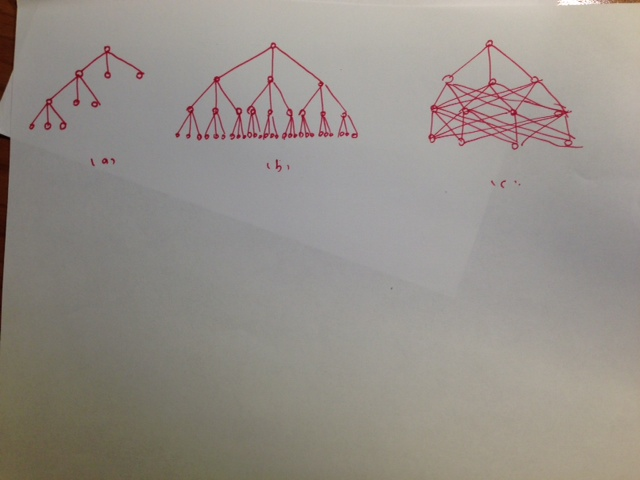
\includegraphics[scale=0.4]{arch.jpg}
\end{center}

The first structure is a partial $m-$tree, which corresponds to the multi-level wavelet or wavelet tight frame transform. The root node represents the input image, (for illustration purpose, the input image has only one channel), applying $m$ filters on the input, we get $m$ sets of wavelet tight frame coefficients. Each set of coefficients is represented using $m$-child nodes. The left most node always represents the low frequency coefficients. To do multi-level transform, we simply apply the same filters on the low frequency coefficients iteratively. Thus, for a level $L$ wavelet tight frame transform, the structure we get a tree of depth $L+1$ . 

This structure arises naturally in wavelet tight frames generated using MRA. The major advantage is the efficient decomposition and reconstruction algorithm. For level-$L$ transform with downsampling, it takes only $\mathcal O(mN)$ operations for the decomposition of a signal of length $N$.
 
Can we extend the previous adaptive construction to multiple levels using this structure? It depends. Such a structure assumes the existence of a single low frequency filter, which our previous construction does not guarantee. However, due to the pleasant surprise described in the previous section, for many datasets, we get a unique low frequency filter automatically. This phenomenon brings us a free lunch. It allows us to carry out multiple level transforms in exactly the same way as we do with pre-defined wavelet tight frames, only with improved performance. Our experience with numerical experiments suggests the rule of thumb, possibly exaggerated: {\color{red}wherever we have used wavelet tight frames for image processing tasks, we can try the adaptive construction using this structure. If we are lucky, we might improve the performance with no additional cost!} \\

The previous structure is great, but requires some luck. Sometimes we get a bunch of filters and no filter is more special than the others. This brings us to the second structure. The first layer is the same as the previous one. Below that, instead of doing transforms on the low frequency coefficients only, we do transforms on all sets of coefficients. As a result, the structure is a full $m$-tree. Apparently, the computational cost is now much larger. It is not appropriate for image compression or restoration tasks, but good for classification tasks. As the computational cost grows exponentially with the number of layers, we have to implement this structure with care and possibly some tricks in practice.  Examples of this structure include the scattering transform proposed by Mallat et.al. \\

It is the intention of creating a compact structure when we have no luck with the first structure that brings us to the third one. The first layer is still the same, below that, the tree structure is replaced by a fully connected structure. Because this structure is more elaborated and less known than the previous two, we shall give the details in the next subsection.















\end{document}